\documentclass[pdf,aspectratio=169]{beamer}
\newcommand{\theme}{define_theme}
\usepackage{xifthen}
\usepackage{listings}
\usepackage[ruled]{algorithm2e}

% Settings for listings package
\definecolor{mygreen}{rgb}{0,0.6,0}
\definecolor{mygray}{rgb}{0.5,0.5,0.5}
\definecolor{mymauve}{rgb}{0.58,0,0.82}
\definecolor{altblue}{rgb}{0.0,0.6,1.0}
\definecolor{lstbg}{gray}{0.9}

\lstset{
  backgroundcolor=\color{lstbg},
  % choose the background color; you must add \usepackage{color} or \usepackage{xcolor}
  basicstyle=\tiny\ttfamily,
  % the size of the fonts that are used for the code
  breakatwhitespace=true,
  % sets if automatic breaks should only happen at whitespace
  breaklines=true,
  % sets automatic line breaking
  captionpos=b,
  % sets the caption-position to bottom
  commentstyle=\color{mygreen},
  % comment style
  deletekeywords={},
  % if you want to delete keywords from the given language
  escapeinside={\#*}{*},
  % if you want to add LaTeX within your code
  extendedchars=true,
  % lets you use non-ASCII characters; for 8-bits encodings only, does not work with UTF-8
  frame=single,
  % adds a frame around the code
  keepspaces=true,
  % keeps spaces in text, useful for keeping indentation of code (possibly needs columns=flexible)
  keywordstyle=\color{blue},
  % keyword style
  %language=c++,
  % the language of the code
  otherkeywords={},
  % if you want to add more keywords to the set
  numbers=left,
  % where to put the line-numbers; possible values are (none, left, right)
  numbersep=5pt,
  % how far the line-numbers are from the code
  numberstyle=\tiny\color{mygray},
  % the style that is used for the line-numbers
  rulecolor=\color{black},
  % if not set, the frame-color may be changed on line-breaks within not-black text (e.g. comments (green here))
  showspaces=false,
  % show spaces everywhere adding particular underscores; it overrides 'showstringspaces'
  showstringspaces=false,
  % underline spaces within strings only
  showtabs=false,
  % show tabs within strings adding particular underscores
  stepnumber=1,
  % the step between two line-numbers. If it's 1, each line will be numbered
  stringstyle=\color{mymauve},
  % string literal style
  tabsize=4,
  % sets default tabsize to 4 spaces
  title=\lstname
  % show the filename of files included with \lstinputlisting; also try caption instead of title
}

\lstdefinelanguage[firedrake]{python}[]{python}{%
  keywordstyle={[2]\color{red}},
   morekeywords={[2]UnitCubeMesh,MeshHierarchy,FunctionSpace,Function,TrialFunction,TestFunction,DirichletBC,SpatialCoordinate,Constant,solve},
  keywordstyle={[3]\color{orange}},
  morekeywords={[3]grad,dx,inner,pi,sin,cos,tan}
}
\lstdefinelanguage[highlighting]{python}[firedrake]{python}{
	moredelim=**[is][{\btHL[fill=red!30,draw=black,thin]}]{`mesh*}{`},
	moredelim=**[is][{\btHL[fill=orange!30,draw=black,thin]}]{`fs*}{`},
	moredelim=**[is][{\btHL[fill=mygreen!30,draw=black,thin]}]{`bcs*}{`},
	moredelim=**[is][{\btHL[fill=blue!30,draw=black,thin]}]{`rhs*}{`},
	moredelim=**[is][{\btHL[fill=violet!30,draw=black,thin]}]{`bilf*}{`}
}

\graphicspath{{figures/}}

\mode<presentation>{
	%firedrake style only if enabled
	\ifthenelse{\equal{\theme}{firedrake}}{
		\usetheme{firedrake}
		\usecolortheme{firedrake}
	}{
		\usetheme{CambridgeUS}
		\usecolortheme{seagull}
	}
}

% Awkward widebar thing... (instead of mathabx)
\makeatletter
\newcommand*\rel@kern[1]{\kern#1\dimexpr\macc@kerna}
\newcommand*\widebar[1]{%
  \begingroup
  \def\mathaccent##1##2{%
    \rel@kern{0.8}%
    \overline{\rel@kern{-0.8}\macc@nucleus\rel@kern{0.2}}%
    \rel@kern{-0.2}%
  }%
  \macc@depth\@ne
  \let\math@bgroup\@empty \let\math@egroup\macc@set@skewchar
  \mathsurround\z@ \frozen@everymath{\mathgroup\macc@group\relax}%
  \macc@set@skewchar\relax
  \let\mathaccentV\macc@nested@a
  \macc@nested@a\relax111{#1}%
  \endgroup
}
\makeatother

% Some tikz magic
\usepackage{tikz}
\usetikzlibrary{arrows}

% Define how TiKZ will draw the nodes
\tikzset{mathterm/.style={draw=none,fill=none,rectangle,inner sep=0pt,anchor=base}}
\tikzstyle{every picture}+=[remember picture]
\everymath{\displaystyle}

\makeatletter

% Designate a term in a math environment to point to
% Syntax: \mathterm[node label]{some math}
\newcommand\mathterm[2][]{%
  \@ifnextchar[{\@mathtermopts{#1}{#2}}{\@mathtermnoopts{#1}{#2}}}
\def\@mathtermnoopts#1#2{%
  \tikz [baseline] { \node [term] (#1) {$#2$}; }}
\def\@mathtermopts#1#2[#3]{%
  \tikz [baseline] { \node [rectangle,inner sep=2pt,rounded corners=2pt,anchor=base,,#3] (#1) {$#2$}; }}

\newcommand\textterm[2][]{%
  \@ifnextchar[{\@texttermopts{#1}{#2}}{\@texttermnoopts{#1}{#2}}}
\def\@texttermnoopts#1#2{%
  \tikz [baseline] { \node [term] (#1) {#2}; }}
\def\@texttermopts#1#2[#3]{%
  \tikz [baseline] { \node [rectangle,inner sep=2pt,rounded corners=2pt,anchor=base,,#3] (#1) {#2}; }}

% A command to draw an arrow from the current position to a labelled math term
% Default color=black, default arrow head=stealth
% Syntax: \indicate[color]{term to point to}[path options]
\newcommand\indicate[2][black]{%
  \tikz [baseline] \node [inner sep=0pt,anchor=base] (i#2) {\vphantom|};
  \@ifnextchar[{\@indicateopts{#1}{#2}}{\@indicatenoopts{#1}{#2}}}
\def\@indicatenoopts#1#2{%
  {\color{#1} \tikz[overlay] \path[line width=1pt,draw=#1,-stealth] (i#2) edge (#2);}}
\def\@indicateopts#1#2[#3]{%
  {\color{#1} \tikz[overlay] \path[line width=1pt,draw=#1,-stealth] (i#2) [#3] edge (#2);}}

\newenvironment{btHighlight}[1][]
{\begingroup\tikzset{bt@Highlight@par/.style={#1}}\begin{lrbox}{\@tempboxa}}
{\end{lrbox}\bt@HL@box[bt@Highlight@par]{\@tempboxa}\endgroup}

\newcommand\btHL[1][]{%
  \begin{btHighlight}[#1]\bgroup\aftergroup\bt@HL@endenv%
}
\def\bt@HL@endenv{%
  \end{btHighlight}%   
  \egroup
}
\newcommand{\bt@HL@box}[2][]{%
  \tikz[#1]{%
    \pgfpathrectangle{\pgfpoint{1pt}{0pt}}{\pgfpoint{\wd #2}{\ht #2}}%
    \pgfusepath{use as bounding box}%
    \node[anchor=base west, fill=orange!30,outer sep=0pt,inner xsep=1pt, inner ysep=0pt, rounded corners=2pt, minimum height=\ht\strutbox+1pt,#1]{\raisebox{1pt}{\strut}\strut\usebox{#2}};
  }%
}
\makeatother

\newcommand{\citehere}[1]{{\footnotesize[#1]}}

\title[Firedrake]{Firedrake}
\subtitle{2021 Code Performance Series}
\author[JB,JF,RNH,SV,CW]{\textbf{Jack Betteridge} \and Joscha Fregin \and Reuben Nixon-Hill \\ Sophia Vorderwuelbecke \and Connor Ward}
\date[20/5/2021]{20${}^\text{th}$ May 2021}

\begin{document}
\maketitle

%%%%%%%%%%%%%%%%%%%%%%%%%%%%%%%%%%%%%%%%%%%%%%%%%%%%%%%%%%%%
\subsection{Overview}
\begin{frame}{What is Firedrake?}
Firedrake (\href{http://firedrakeproject.org/}{\texttt{firedrakeproject.org/}}) is
\begin{itemize}
	\item high-level
	\item high-productivity
	\item Python based
	\item code generation framework
\end{itemize}
for the specification and solution of PDEs using the finite element method. 

Parallelism is achieved through MPI.
\end{frame}

%%%%%%%%%%%%%%%%%%%%%%%%%%%%%%%%%%%%%%%%%%%%%%%%%%%%%%%%%%%%
\subsection{Profiling}
\begin{frame}[fragile]{Why is profiling difficult?}
\begin{columns}[T]
\begin{column}[T]{0.45\textwidth}
Invocation:
\begin{lstlisting}[language={bash}]
mpiexec -n 16 python poisson.py
\end{lstlisting}

Example code solving Poisson's equation\\
Notice:
\begin{itemize}
	\item No compiling
	\item No MPI
	\item No C/C++/FORTRAN
\end{itemize}
\end{column}
\begin{column}[T]{0.45\textwidth}
\vspace{-3em}
\begin{lstlisting}[language={[highlighting]python}]
from firedrake import *

N = 12
mesh = UnitCubeMesh(N, N, N)
hierarchy = MeshHierarchy(mesh, 1)
mesh = hierarchy[-1]

fs*degree = 3
V = FunctionSpace(mesh, "CG", degree)
u = TrialFunction(V)
v = TestFunction(V)

bcs = DirichletBC(V, zero(), (1, 2, 3, 4, 5, 6))

x, y, z = SpatialCoordinate(mesh)
a = Constant(1)
b = Constant(2)

rhs*f = -pi**2 / 2
rhs*f *= 2*cos(pi*x) - cos(pi*x/2)
    rhs* - 2*(a**2 + b**2)*sin(pi*x)*tan(pi*x/4)
rhs*f *= sin(a*pi*y)*sin(b*pi*z)

a = dot(grad(u), grad(v))*dx
bilf*L = f*v*dx

solver_parameters = {...}
u = Function(V)
solve(a == L, u, bcs=bcs, solver_parameters=solver_parameters)
\end{lstlisting}
\end{column}
\end{columns}
\end{frame}

\begin{frame}
\begin{figure}
	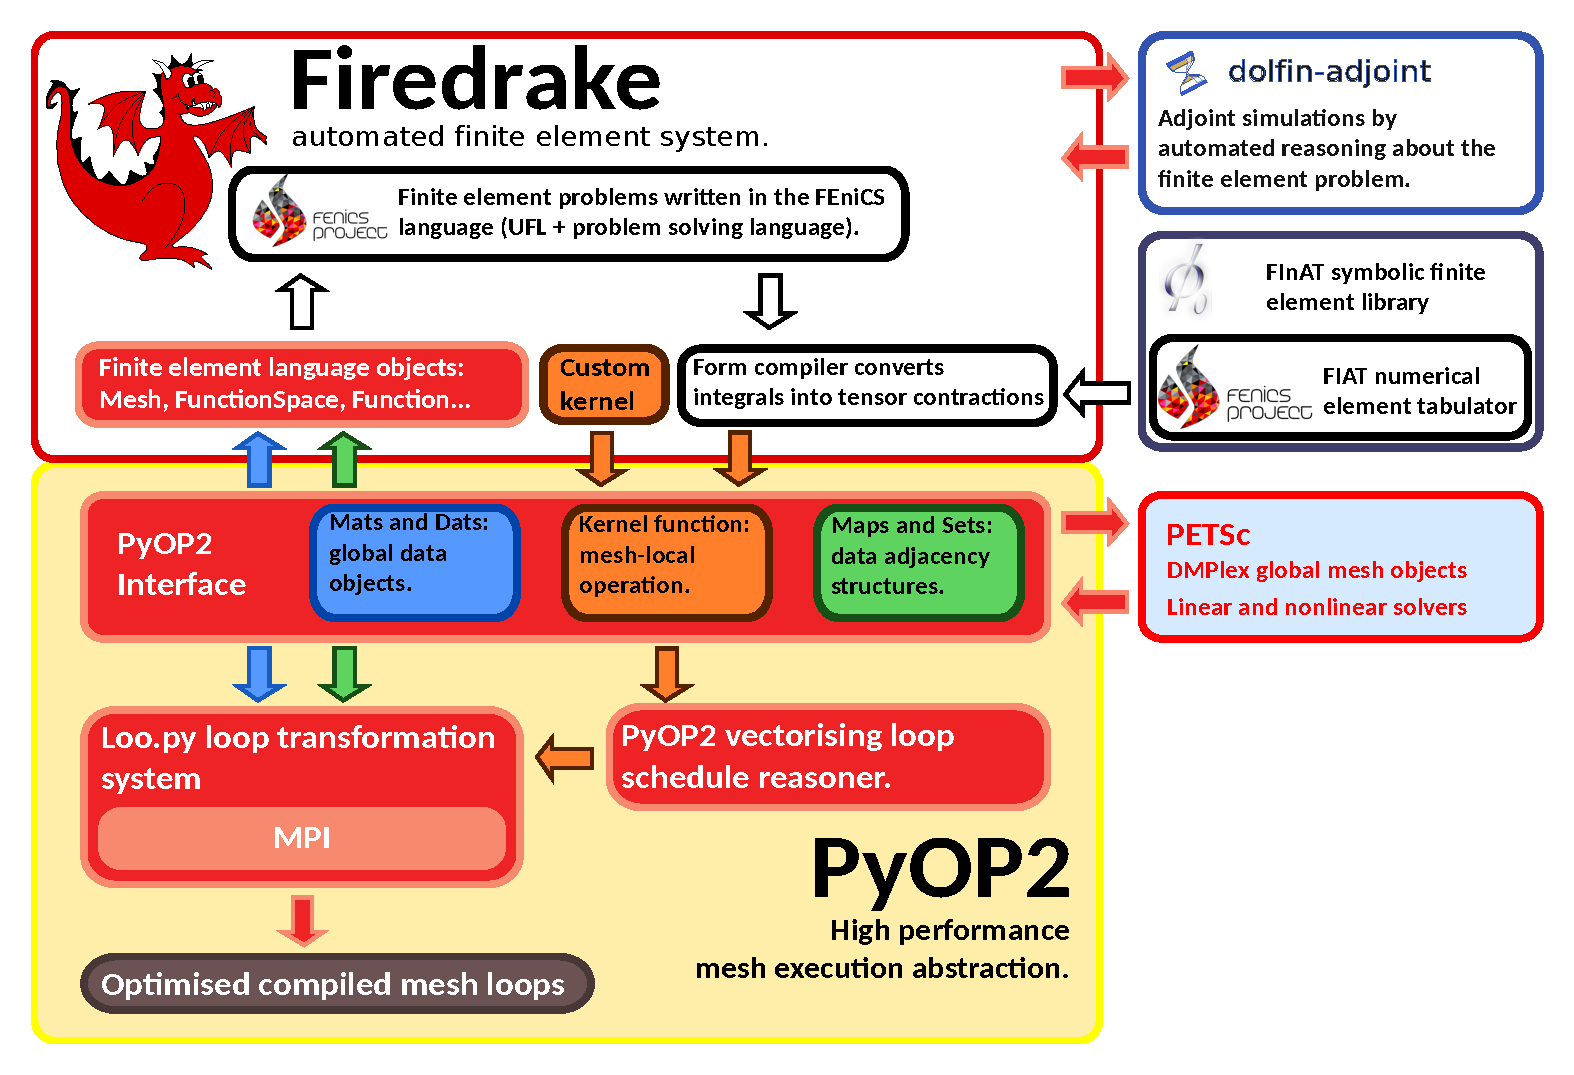
\includegraphics[width=0.8\textwidth]{firedrake_diagram.pdf}
\end{figure}
\end{frame}

%%%%%%%%%%%%%%%%%%%%%%%%%%%%%%%%%%%%%%%%%%%%%%%%%%%%%%%%%%%%
\subsection{Commercial tools}
\begin{frame}[fragile]{VTune and DDT}
Intel VTune
\begin{lstlisting}
> mpiexec -n 2 \
    aps -r vtune --collection-mode=mpi \
        python simple.py
python3: symbol lookup error: /cosma/local/intel/Parallel_Studio_XE_2019/vtune_amplifier_2019.4.0.597835/lib64/libmps.so: undefined symbol: PMPI_Initialized
aps Error: Cannot run: python3 simple.py
\end{lstlisting}

ARM MAP / Allinea DDT
\begin{lstlisting}
> perf-report \
    mpiexec -n 16 \
        python poisson.py
\end{lstlisting}
Works! But we did have to recompile Python from scratch...
\end{frame}

\begin{frame}
\begin{figure}
	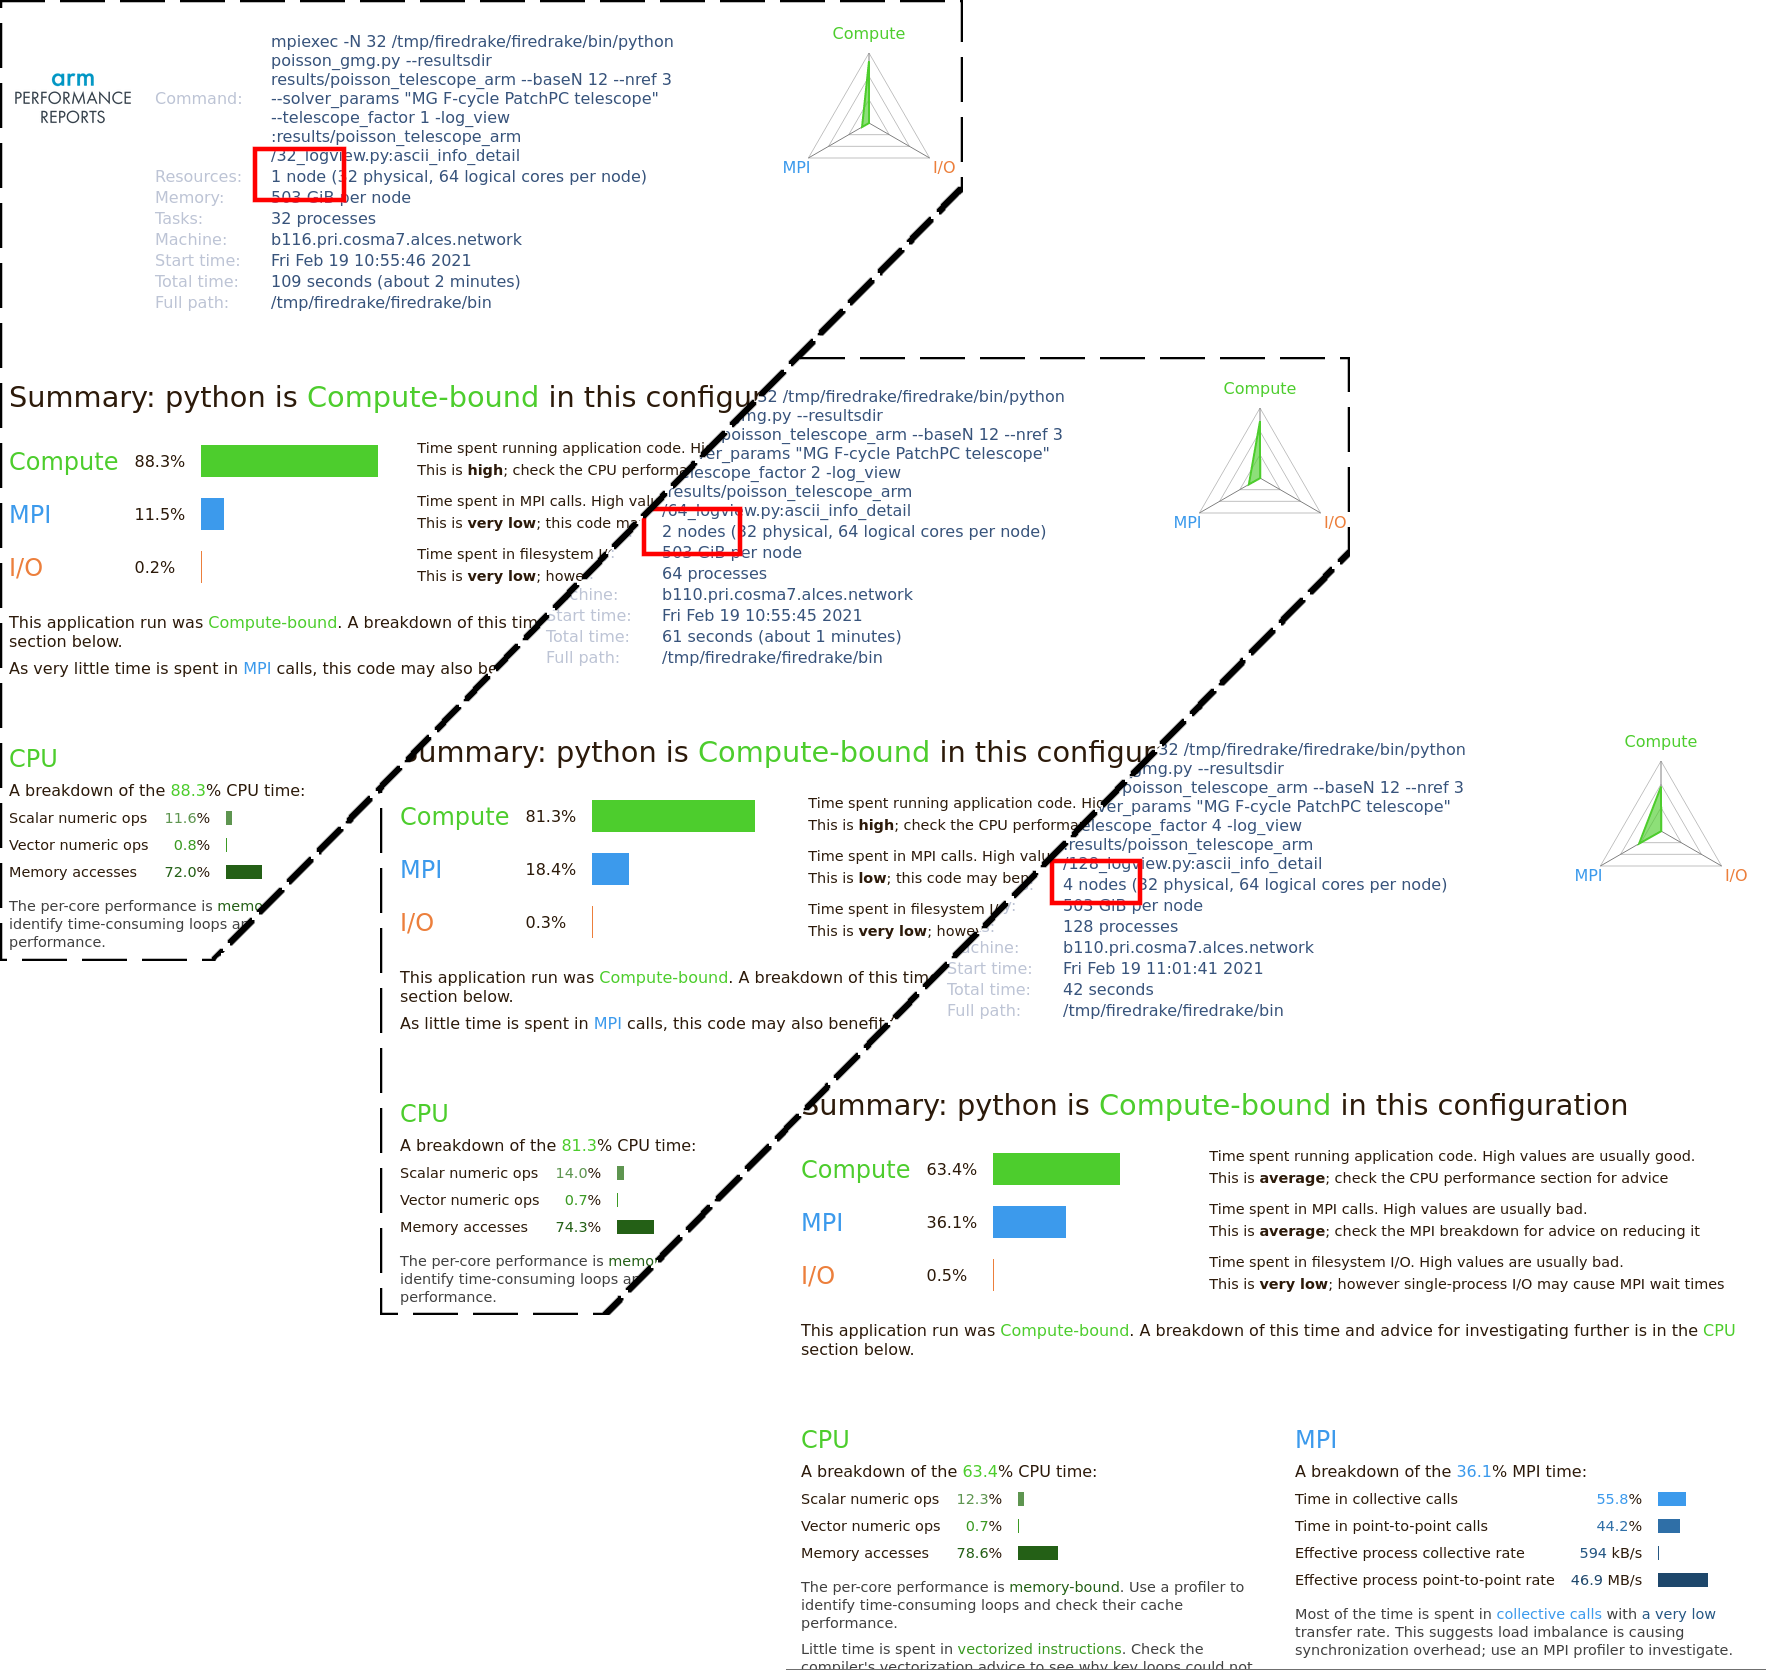
\includegraphics[width=\textheight]{ddt_all.png}
\end{figure}
\end{frame}

\begin{frame}[fragile]{SCORE-P}
We like SCORE-P, it has Python bindings!
\begin{lstlisting}
> mpiexec -n 16 \
    python -m scorep \
        --mpp=mpi --instrumenter-type=cProfile \
            poisson_gmg.py
\end{lstlisting}
We had to recompile SCORE-P from scratch too, but this issue has since been fixed.
\end{frame}

\begin{frame}[fragile]
The filter is essential
\begin{lstlisting}
SCOREP_REGION_NAMES_BEGIN
  EXCLUDE
    argparse*
    importlib*
    matplotlib*
    sympy*
    ufl*
    sre_parse:*
    sre_compile:*
    importlib.*
    zipfile:*
    pkg_resources:*
    pkg_resources.:*
    pathlib:*
    enum:*
SCOREP_REGION_NAMES_END
\end{lstlisting}
\vspace{-2em}
Careful balance to strike:
\begin{itemize}
	\item Call stack is deep
	\item Autogenerated code is at the bottom (can't \verb`INCLUDE` either)
	\item Increasing profiling makes file size unmanagable
\end{itemize}
\end{frame}

\begin{frame}
\begin{figure}
	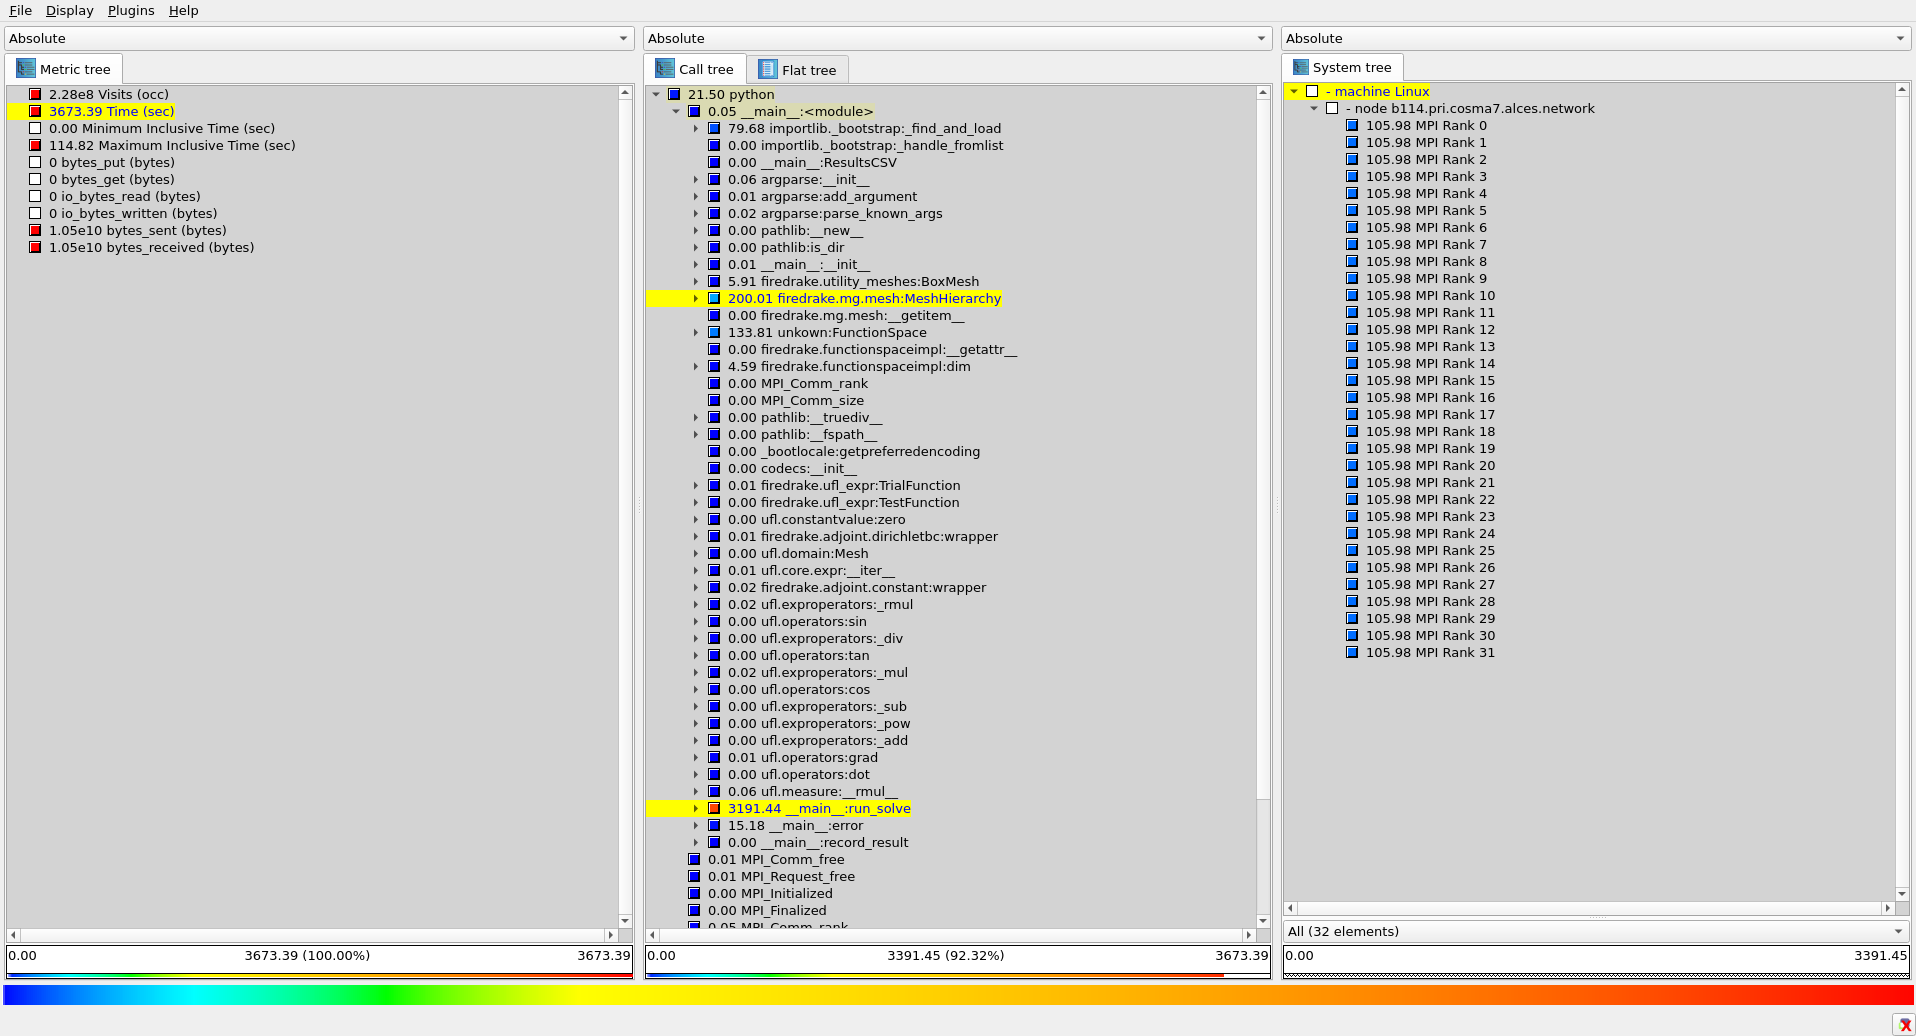
\includegraphics[width=\textwidth]{cube.png}
\end{figure}
\end{frame}

\begin{frame}{Flamegraph tool}
We can get a good visual representation of how the code is performing by plotting a flamegraph of PETSc and PyOP2 calls
\begin{figure}
	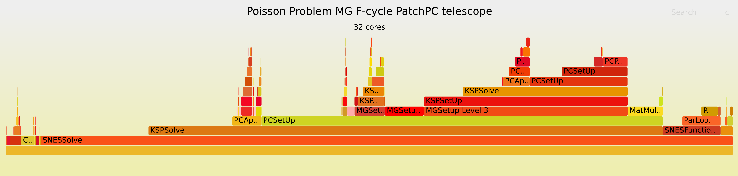
\includegraphics[width=0.8\textwidth]{32_flame.pdf}
	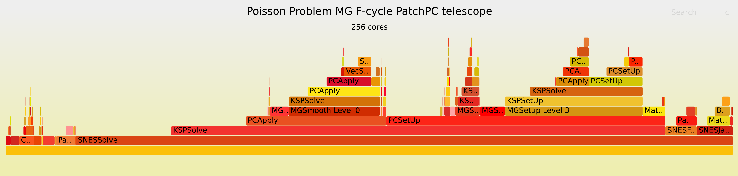
\includegraphics[width=0.8\textwidth]{256_flame.pdf}
\end{figure}
\end{frame}

\begin{frame}{PETSc profiling}
PETSc also displays profiling information for all of its calls, and raw information can be displayed at the end of a simulation, or plotted
\begin{figure}
	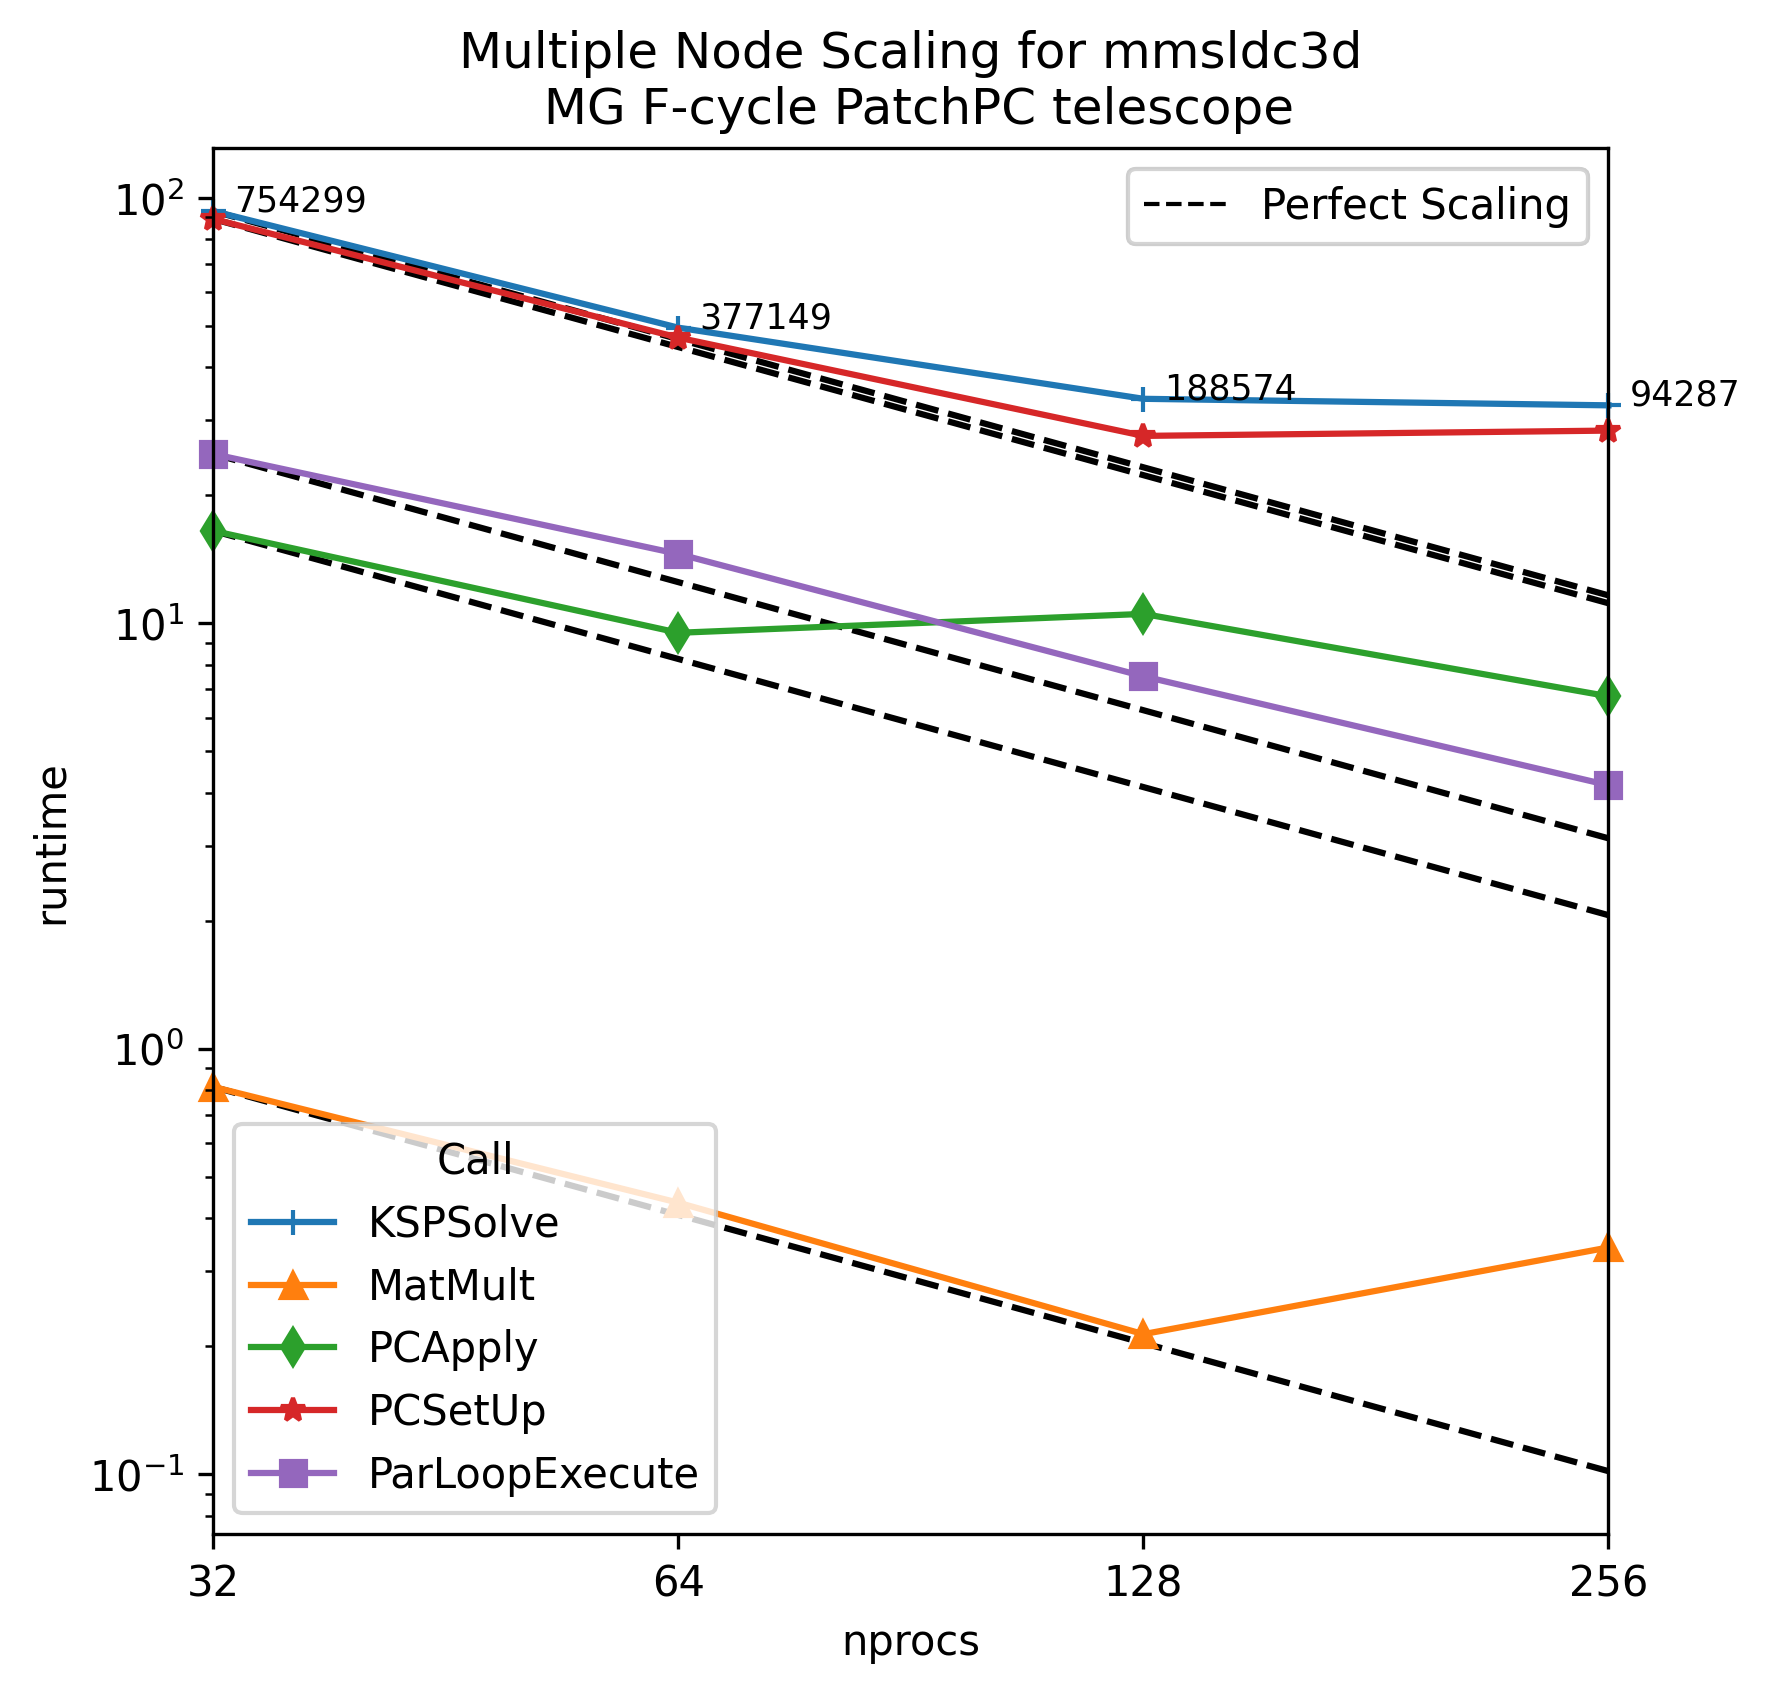
\includegraphics[width=0.4\textwidth]{main_stage.png}
	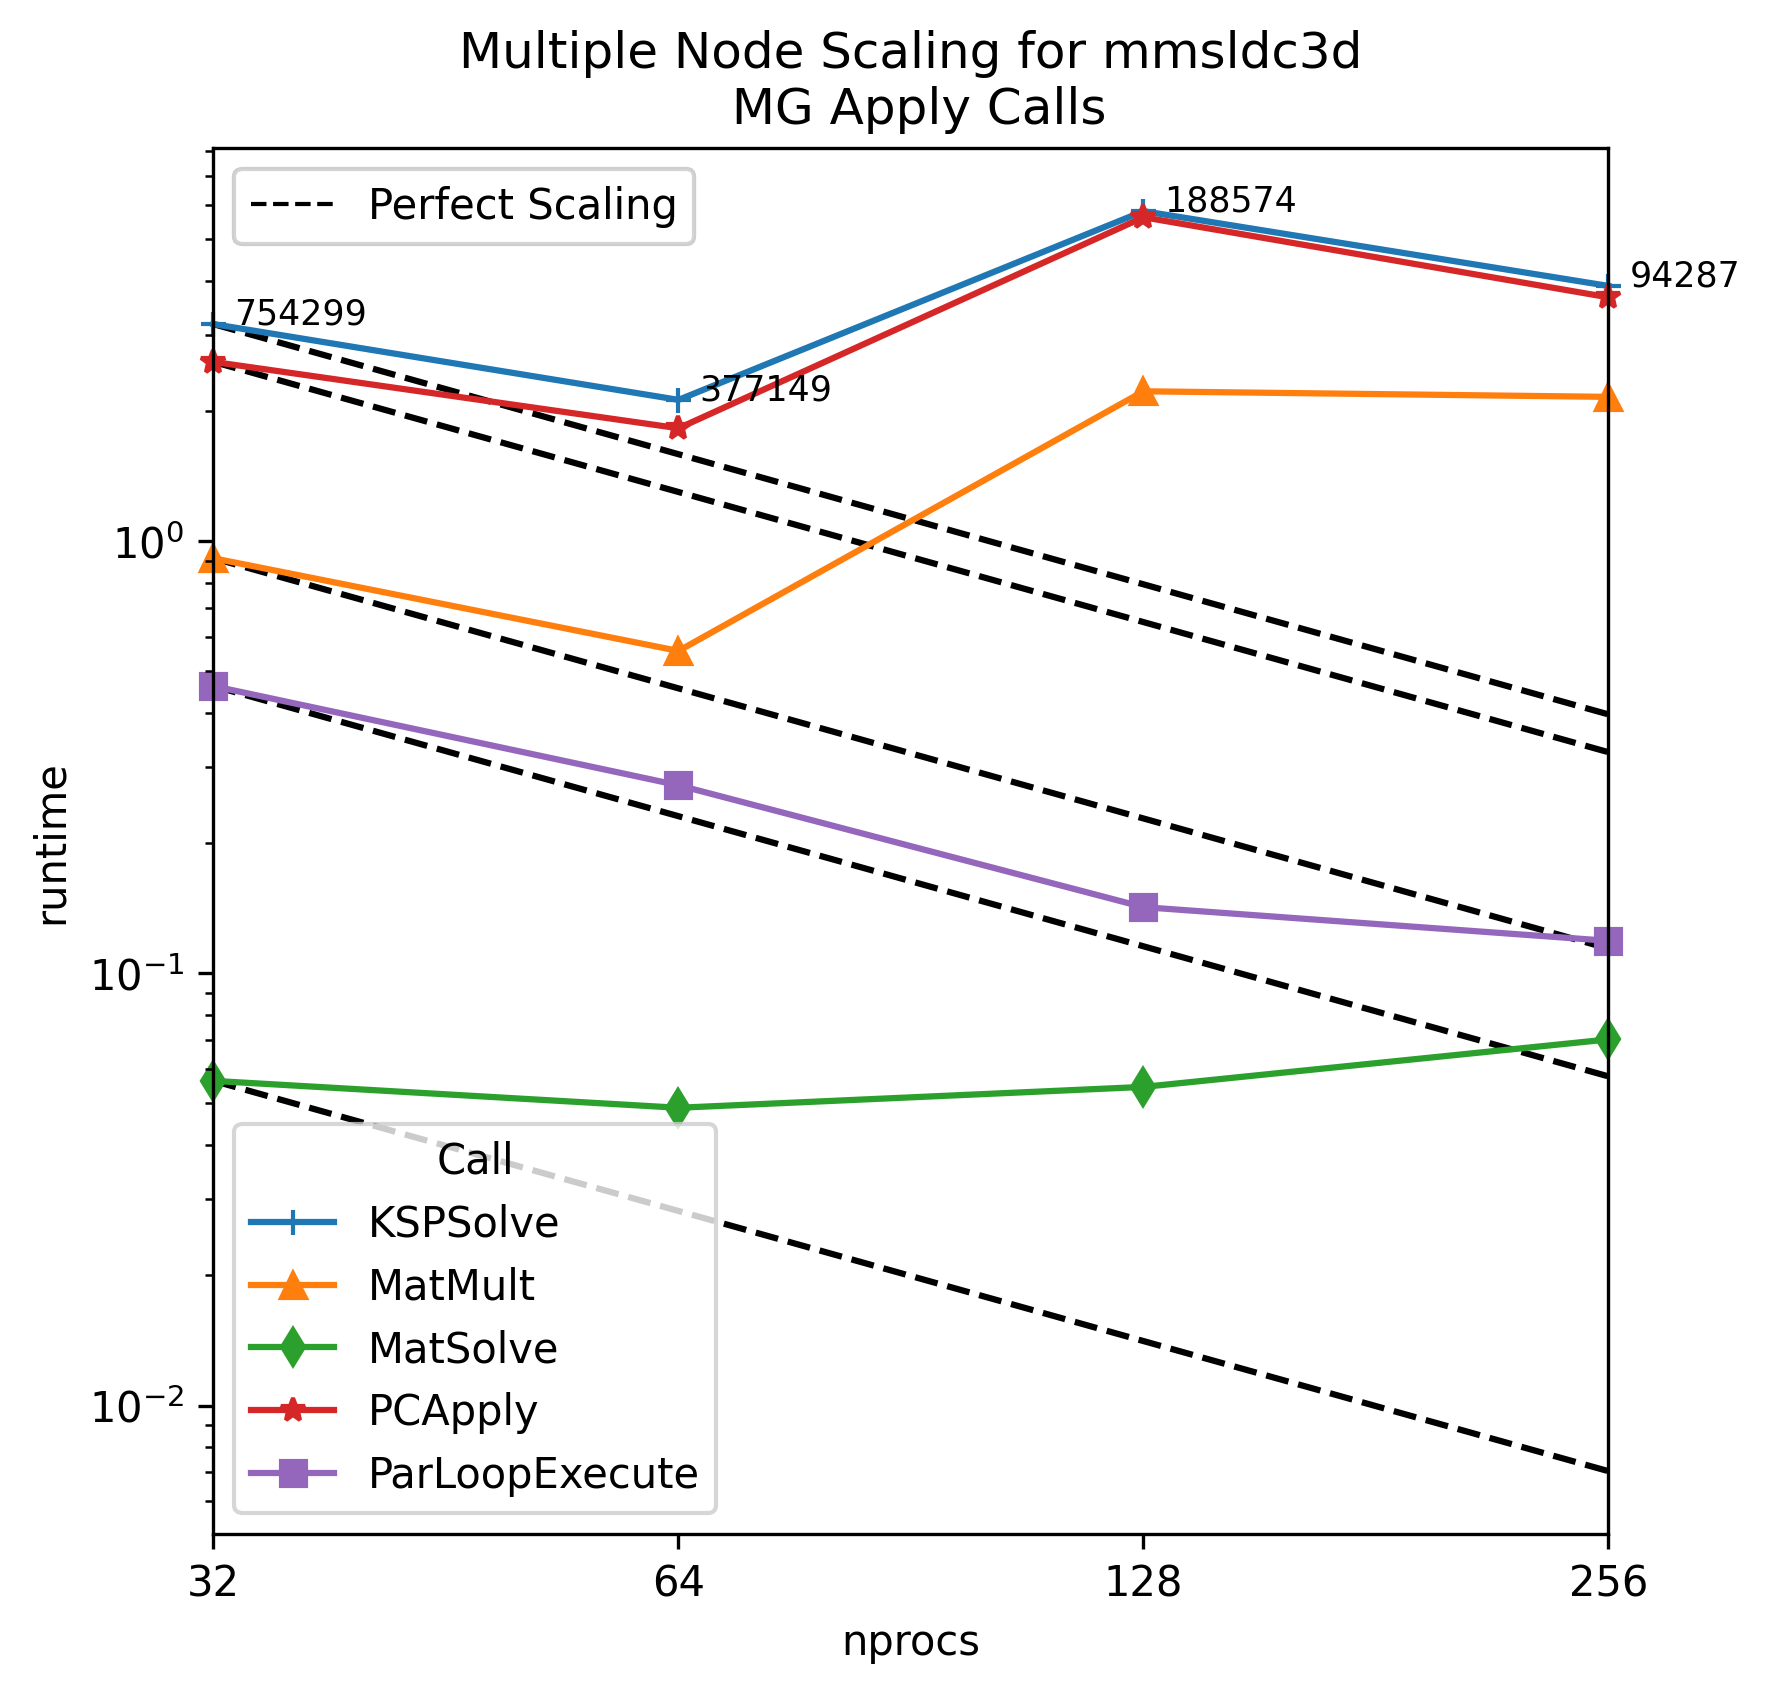
\includegraphics[width=0.4\textwidth]{mgapply.png}
\end{figure}
\end{frame}

\begin{frame}{Vampir and Scalasca}
\begin{itemize}
	\item Vampir: looks good, but using it forwarded over ssh was a pain.
	\item Proprietary nature of the tool means we are unlikely to use it.
	\item Would be nice if Cube had a tool for visualising traces (already available?)
	\item Haven't had much chance to play with Scalasca from the previous session.
\end{itemize}
\end{frame}

\begin{frame}{Summary}
\begin{itemize}
	\item Adding more profiling hooks to the Firedrake code base
	\item Code generation (at least the way we do it) causes issues for many of the tools we've used
	\item SCORE-P + Cube viewer were really useful once we got them working
	\item Would be nice if profiling wasn't so oriented towards monolithic compiled executables (or at least considered other cases)
\end{itemize}
\end{frame}

\end{document}